\documentclass[a4paper,12pt]{article} % тип документа

\usepackage{tikz}
\usepackage[T2A]{fontenc}			% кодировка
\usepackage[utf8]{inputenc}			% кодировка исходного текста
\usepackage[english,russian]{babel}	% локализация и переносы
\usepackage{amsfonts,longtable}

% Математика
\usepackage{amsmath,amsfonts,amssymb,amsthm,mathtools} 


\usepackage{wasysym}

\title{Лабораторная работа 1.2.3 по курсу \\ "Общая физика"  \\ 
\vspace{0.2cm}
\vspace{4.5cm}
 \LARGE{\textbf{Определение моментов инерции твердых тел с помощью трифилярного подвеса}}\vspace{5.5cm}}
\date{30.11.2018}
\usepackage{tikz}
\author{\vspace{0.2cm}Баринов Леонид}

\begin{document}
\maketitle
\newpage
\section{Аннотация}
В работе будет измерен момент инерции ряда тел и проведено сравнение результатов с расчетами по теоретическим формулам. Будет осуществлена проверка аддитивности моментов инерции и справедливости формулы Гюйгенса-Штейнера.
\section{Теоретические сведения}
Инерционность при вращении тела относительно оси определяется моментом инерции тела относительно этой оси. Момент инерции твердого тела относительно неподвижной оси вращения вычисляется по формуле:
\begin{equation}
I = \int r^2dm
\end{equation}
Здесь $r$ -- расстояние элемента массы тела $dm$ от оси вращения. Интегрирование проводится по всей массе тела $m$.
\begin{figure}[h]
\centering
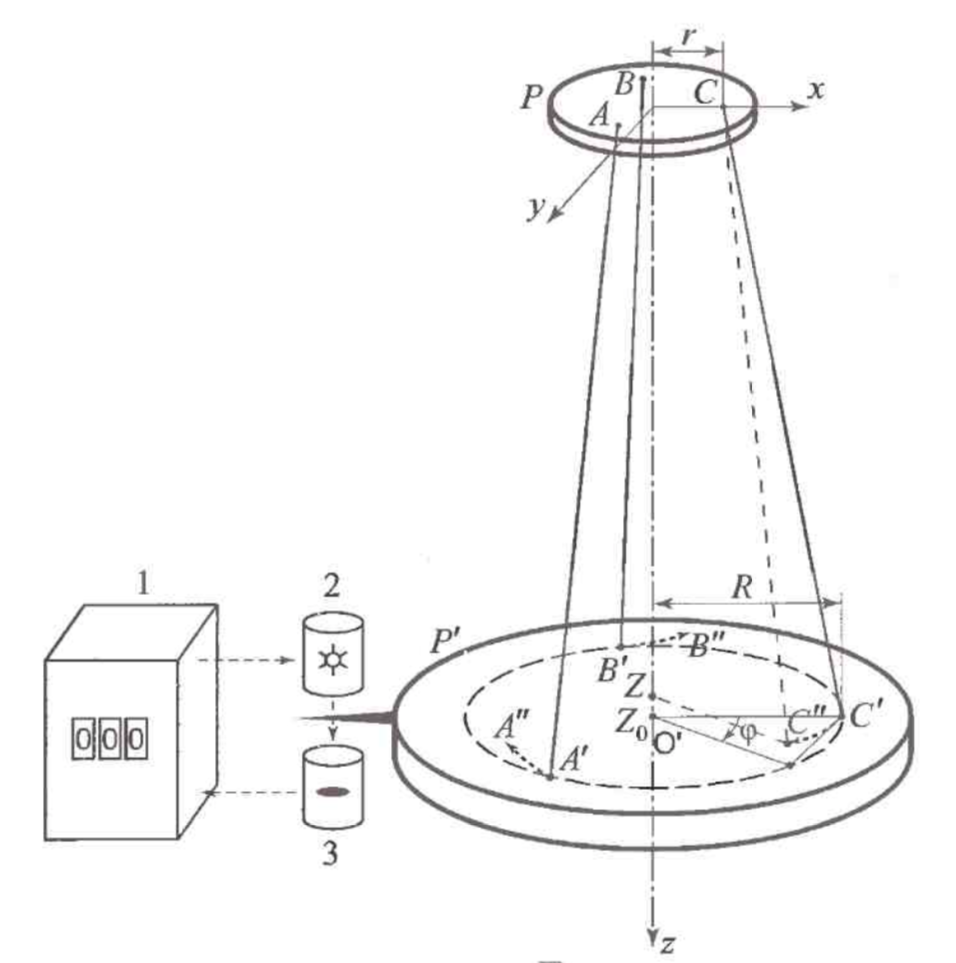
\includegraphics[scale=0.5]{1}
\caption{Трифилярный подвес}
\end{figure}

Для однородных тел известной плотности при заданных размерах и достаточно простой форме момент инерции можно вычислить. Для неоднородных тел и тел сложной формы момент инерции можно определить экспериментально. Удобно использовать устройство, показанное на Рис. 1 и называемое трифилярным подвесом. Оно состоит из укрепленной на некоторой высоте неподвижной платформы $P$, и подвешенной к ней на трех симметрично расположенных нитях $AA', BB'$ и $CC'$ вращающейся платформы $P'$.

Платформа $P$ укреплена на кронштейне и снабжена рычагом (на рисунке не показан), при помощи которого в системе можно создать крутильные колебания путем небольшого поворота верхней платформы. Лучше поворачивать верхнюю платформу, укрепленную на неподвижной оси, чем подвешенную на нитях нижнюю, так как нижнюю платформу трудно закрутить не вызвав ее раскачиваний, подобных движению маятника, учет которых сильно усложнил бы расчеты. После поворота, вызывающего крутильные колебания, верхняя платформа остается неподвижной в течение всего процесса колебаний. После того, как нижняя платформа $P'$ оказывается повернутой на угол $\varphi$ относительно верхней платформы $P$, возникает момент сил, стремящийся вернуть нижнюю платформу в положение равновесия, при котором относительный поворот отсутствует. Но в положении равновесия платформа не останавливается, так как имеет угловую скорость (кинетическую энергию вращения). В результате платформа совершает крутильные колебания.

Если пренебречь потерями энергии на трение (о воздух и в креплениях нитей), то уравнение сохранения энергии при колебаниях можно записать следующим образом:
\begin{equation}
\frac{I\dot{\varphi^2}}{2} + mg(z_0-z) = E
\end{equation} 

Здесь $I$ -- момент инерции платформы вместе с исследуемым телом, $m$ -- масса платформы с телом, $\varphi$ -- угол поворота платформы от положения равновесия системы, точкой обозначена производная по времени (угловая скорость), $z_0$ -- координата по вертикали центра нижней платформы $O'$ при равновесии ($\varphi$ = 0), $z$ -- координата той же точки при некотором угле поворота $\varphi$. Первый член в левой части уравнения -- кинетическая энергия вращения, второй член -- потенциальная энергия в поле тяжести, $E$ -- полная энергия системы (платформы с телом).

Отметим, что, как показывает соотношение (2), возвращающая сила возникает благодаря силе тяжести.

Воспользуемся системой координат $x, y, z$, связанной с верхней платформой, как показано на рис. 1. Координата верхнего конца одной из нитей подвеса точки $C$ в этой системе -- $(r, 0, 0)$. Нижний конец данной нити $C'$, находящийся на нижней платформе, при равновесии имеет координаты $(R, 0, z_0)$, а при повороте платформы на угол $\varphi$ эта точка переходит в $C''$ с координатами $(R\cos\varphi, R\sin\varphi, z)$. Расстояние между точками $C$ и $C''$ равно длине нити $L$. Поэтому:
\begin{equation}
(R\cos\varphi-r)^2 + R^2\sin^2\varphi + z^2 = L^2
\end{equation}
Учитывая, что при малых углах поворота $\cos\varphi\approx 1 - \frac{\varphi}{2}$, получаем 
\begin{equation}
z^2 = L^2 - R^2 - r^2 + 2Rr\cos\varphi = x_0^2 - 2Rr(1-\cos\varphi) \approx z_0^2 - Rr\varphi^2
\end{equation}
Извлекая из (4) квадратный корень и учитывая малость угла $\varphi$, имеем
\begin{equation}
z \approx \sqrt{z_0^2 - Rr\varphi^2}\approx z_0\sqrt{1 - \frac{Rr\varphi^2}{z_0^2}}\approx z_0 - \frac{Rr\varphi^2}{2z_0}
\end{equation}
Подставляя это значение $z$ в уравнение (2), получаем
\begin{equation}
\frac{1}{2}I\dot\varphi^2 + mg\frac{Rr}{2z_0}\varphi^2 = E
\end{equation}

Дифференцируя по времени и сокращая на $\dot{\varphi}$, находим уравнение крутильных колебаний системы:
\begin{equation}
I\ddot{\varphi}+mg\frac{Rr}{z_0}\varphi = 0
\end{equation}
Производная по времени от $E$ равно нулю, так как потерями энергии на трение, как уже было сказано выше, пренебрегаем.

Решение этого уравнения, как нетрудно убедиться простой подстановкой, имеет вид
\begin{equation}
\varphi = \varphi_0\sin\left(\sqrt{\frac{mgRr}{Iz_0}}t+\theta\right)
\end{equation}
Здесь амплитуда $\varphi_0$ и фаза $\theta$ колебаний определяются начальными условиями. Период крутильных колебаний нашей системы равен
\begin{equation}
T = 2\pi\sqrt{\frac{Iz_0}{mgRr}}
\end{equation}
Обратим внимание на то, что из этой формулы при $r = R$ и $I = mR^2$ (тонкое кольцо) получаем формулу для математического маятника.

Из (9) находим формулу для определения момента инерции:
\begin{equation}
I = \frac{mgRrT^2}{4\pi^2z_0}
\end{equation}

Учитывая, что параметры установки $R$, $r$ и $z_0$ при проведении опытов не меняются, удобно переписать последнее уравнение следующим образом:
\begin{equation}
I = kmT^2
\end{equation}
Здесь $k = \frac{gRr}{4\pi^2z_0}$ -- величина, постоянная для данной установки.

Таким образом, полученные формулы позволяют определить момент инерции платформы с телом и отдельно платформы по соответствующим периодам крутильных колебаний. Затем вычисляем момент инерции тела, пользуясь аддитивностью, в справедливости которой можно убедиться, проведя измерения сначала для каждого из двух тел отдельно, а затем для обоих тел вместе.

При выводе формул предполагалось, что малы необратимые потери энергии, связанные с трением, то есть мало затухание колебаний. О затухании колебаний можно судить, сравнивая время $\tau$ уменьшения амплитуды колебаний в 2-3 раза с периодом колебаний $T$. Необратимыми потерями энергии можно пренебречь, если выполняется условие 
\begin{equation}
\tau \gg T
\end{equation}

В данной работе рекомендуется период колебаний определять с относительной погрешность $0,5\%$. Число колебаний, по которым надо вычислять период, определяется этой погрешностью и погрешностью измерения времени.

Для счета числа колебаний используется счетчик, состоящий из осветителя (2), фотоэлемента (3) и пересчётного устройства (1) (см Рис. 1). Легкий лепесток, укрепленный на платформе, при колебаниях пересекает световой луч дважды за период. Соответствующие сигналы от фотоэлемента поступают на пересчетное устройство.
\section{Оборудование и инструментальные погрешности}
В работе используются: трифилярный подвес (см. Рис. 1), секундомер, счетчик числа колебаний, набор тел, момент инерции которых надлежит измерить -- диск, полый цилиндр. Для удобства на платформе трифилярного подвеса нанесен ряд концентрических окружностей.\\
Параметры трифилярного подеса (см. Рис. 1)
\[ R = (115,4\pm0,5)\text{мм}\]
\[r = (30,5\pm 0,3)\text{мм}\]\\
Масса платформы:
\[m = (993,5\pm0,3)\text{г}\]
Расстояние от центра трех креплений до края платформы:
\[z = 215\pm0,5\text{см}\]
Посчитаем $z_0$ по теореме Пифагора:
\[z_0 = \sqrt{z^2 - R^2} = 2146,9\text{мм}\]
Масса полого цилиндра:
\[m_\text{ц} = 981,7\text{г}\]
Внешний радиус полого цилиндра:
\[R_\text{ц} = (84,0\pm0,1)\text{мм}\]
"Толщина" полого цилиндра:
\[\Delta l = (0,53\pm 0,1)\text{мм}\]
Масса диска:
\[m_\text{д} = 580,6\text{г}\]
Радиус диска:
\[R_\text{д} = (85\pm0,1)\text{мм}\]
Масса первого полуцилиндра:
\[m_1 = 764,1\text{г}\]
Масса второго полуцилиндра:
\[m_2 = 764,5\text{г}\]
\section{Результаты измерений и обработка данных}
Вычислим константу установки $k$, входящую в формулу (11), и ее погрешность
\[k = \frac{gRr}{4\pi^2z_0}\]
\[k = 406,4\pm 4,4\frac{\text{мм}^2}{\text{c}^2}\]
Проведем серию измерений периода времени колебаний платформы для определения ее момента инерции. Результаты запишем в Таблицу 1. $n$ - число полуколебаний.
\newpage
\begin{table}[h]
\centering
\begin{tabular}{|c|c|c|c|}
\hline
$\text{№}$ & $n$  & $t, c$ & $T, c$       \\ \hline
1  & 28   & 61,69  & 4,41 \\ \hline
2  & 27   & 59,384 & 4,40 \\ \hline
3  & 28   & 62,271 & 4,45 \\ \hline
4  & 27   & 60,227 & 4,46 \\ \hline
5  & 27   & 60,167 & 4,46 \\ \hline
6  & 27   & 59,75  & 4,43 \\ \hline
7  & 28   & 61,97  & 4,43 \\ \hline
8  & 31   & 68,667 & 4,43 \\ \hline
9  & 28   & 61,925 & 4,42 \\ \hline
10 & 28   & 62,086 & 4,43 \\ \hline
\end{tabular}
\caption{Период колебаний ненагруженной платформы}
\end{table}
Посчитаем среднее значение периода колебаний платформы и определим ее погрешность.
\[T_\text{ср} = (4,431\pm0,019)\text{с}\]
Относительная погрешность:
\[\sigma_{T_\text{ср}} = 0,43\%\]
Будем использовать эту относительную погрешность при определении погрешности периодов колебаний других тел.
Посчитаем момент инерции платформы по формуле (11):
\[I = kmT^2\]
\[I = (7,9\pm0,1)\text{г}\cdot \text{м}^2\]
Проведем серию измерений периода колебаний платформы с находящимся на ней полым цилиндром. Результаты занесем в Таблицу 2.
\begin{table}[h]
\centering
\begin{tabular}{|c|c|c|c|}
\hline
$\text{№}$ & $n$  & $t, c$ & $T, c$   \\ \hline
1 & 29 & 61,712 & 4,26 \\ \hline
2 & 32 & 67,89  & 4,24 \\ \hline
3 & 29 & 61,718 & 4,26 \\ \hline
\end{tabular}
\caption{Период колебаний платформы с находящимся на ней полым цилиндром}
\end{table}

Посчитаем среднее значение периода колебаний. Систематической погрешностью можно пренебречь, будем учитывать относительную погрешность $\sigma_{T_\text{ср}}$
\[T_\text{ц} = (4,252\pm0,018)\text{с}\]
Посчитаем момент инерции платформы с полым цилиндром по формуле (11):
\[I_\text{ц+п} = (14,51\pm 0,18)\text{г}\cdot \text{м}^2\]
Исходя из аддитивности момента инерции найдем момент инерции полого цилиндра:
\[I_\text{ц} = I_\text{ц+п} - I = (6,58\pm 0,26)\text{г}\cdot \text{м}^2\]
Проведем серию измерений периода колебаний платформы с находящимся на ней диском. Результаты занесем в Таблицу 3.
\begin{table}[h]
\centering
\begin{tabular}{|c|c|c|c|}
\hline
$\text{№}$ & $n$  & $t, c$ & $T, c$   \\ \hline
1 & 31 & 61,336 & 3,96 \\ \hline
2 & 31 & 61,008 & 3,94 \\ \hline
3 & 31 & 60,988 & 3,93 \\ \hline
\end{tabular}
\caption{Период колебаний платформы с находящимся на ней диском}
\end{table}

Посчитаем среднее значение периода колебаний. Систематической погрешностью можно пренебречь, будем учитывать относительную погрешность $\sigma_{T_\text{ср}}$
\[T_\text{д} = (3,943\pm0,018)\text{с}\]
Посчитаем момент инерции платформы с диском по формуле (11):
\[I_\text{д+п} = (9,94\pm 0,12)\text{г}\cdot \text{м}^2\]
Исходя из аддитивности момента инерции найдем момент инерции диска:
\[I_\text{д} = I_\text{д+п} - I = (2,02\pm 0,22)\text{г}\cdot \text{м}^2\]
Проведем серию измерений периода колебаний платформы с находящимся на ней диском и полым цилиндром. Результаты занесем в Таблицу 4.

\begin{table}[!h]
\centering
\begin{tabular}{|c|c|c|c|}
\hline
$\text{№}$ & $n$  & $t, c$ & $T, c$   \\ \hline
1 & 31 & 62,196 & 4,01 \\ \hline
2 & 31 & 62,202 & 4,01 \\ \hline
3 & 31 & 62,159 & 4,01 \\ \hline
\end{tabular}
\caption{Период колебаний платформы с находящимся на ней диском и полым цилиндром}
\end{table}

Посчитаем среднее значение периода колебаний. Систематической погрешностью можно пренебречь, будем учитывать относительную погрешность $\sigma_{T_\text{ср}}$
\[T_\text{д+ц} = (4,012\pm0,017)\text{с}\]
Посчитаем момент инерции платформы с полым цилиндром и диском по формуле (11):
\[I_\text{д+п+ц} = (16,72\pm 0,21)\text{г}\cdot \text{м}^2\]
Исходя из аддитивности момента инерции найдем момент инерции полого цилиндра и диска:
\[I_\text{д+ц} = I_\text{д+п+ц} - I = (8,8\pm 0,3)\text{г}\cdot \text{м}^2\]
Почситаем значения моментов инерции тел исходя исходя из теоритичских формул:
Момент инерции полого цилиндра:
\[I_\text{ц}^\text{т} = m_\text{ц}\frac{R_\text{ц}^2+(R_\text{ц}-\Delta l)^2}{2}\]
\[I_\text{ц}^\text{т} = (6,833\pm0,003)\text{г}\cdot \text{м}^2\]
Момент инерции диска:
\[I_\text{д}^\text{т} = \frac{1}{2}m_\text{д}R_\text{д}\]
\[I_\text{ц}^\text{т} = (2,10\pm0,002)\text{г}\cdot \text{м}^2\]
Поместим на платформу диск, разрезанный до диаметру. Постепенно раздвигая половинки диска так, чтобы их общий центр масс все время оставался на оси вращения платформы (Рис. 2), снимаем зависимость момента инерции такой системы $I_c$ от расстояния $h$ каждой из половинок до оси вращения (центра платформы). Результаты занесем в Таблицу 5. $n$ - число полуколебаний. $T$ -- период колебаний. $I$ -- момент инерции двух полуцилиндров. $I = km_c T^2 - I_c$, $m_c = m+m_1+m_2$
\begin{figure}[h]
\centering
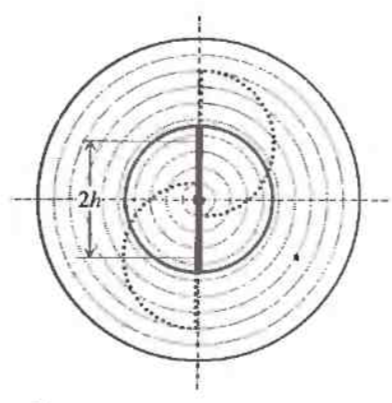
\includegraphics[scale=0.5]{2}
\caption{Расположение тел на платформе}
\end{figure}
\newpage
\begin{table}[h]
\centering
\begin{tabular}{|c|c|c|c|c|c|c|c|c|}
\hline
$\text{№}$ & $n$  &$t, c$  & $h,\text{см}$ & $T, c$     & $I$     &   $\sigma_I$   &    $h^2, \text{см}^2$   & $\sigma_{h^2}$    \\ \hline
1  & 40 & 60,777 & 0     & 3,04 & 1,54 & 0,02 & 0     & 0,1 \\ \hline
2  & 40 & 61,089 & 0     & 3,05 & 1,63 & 0,02 & 0     & 0,1 \\ \hline
3  & 43 & 66,17  & 1     & 3,08 & 1,78 & 0,02 & 1     & 0,1 \\ \hline
4  & 40 & 61,367 & 1     & 3,07 & 1,72 & 0,02 & 1     & 0,1 \\ \hline
5  & 39 & 61,216 & 2     & 3,14 & 2,17 & 0,02 & 4     & 0,1 \\ \hline
6  & 38 & 60,792 & 2,5   & 3,20 & 2,57 & 0,03 & 6,25  & 0,1 \\ \hline
7  & 37 & 60,111 & 3     & 3,25 & 2,89 & 0,03 & 9     & 0,1 \\ \hline
8  & 37 & 61,734 & 3,5   & 3,34 & 3,49 & 0,04 & 12,25 & 0,1 \\ \hline
9  & 36 & 61,793 & 4     & 3,43 & 4,15 & 0,04 & 16    & 0,1 \\ \hline
10 & 35 & 61,68  & 4,5   & 3,52 & 4,80 & 0,05 & 20,25 & 0,1 \\ \hline
11 & 35 & 63,098 & 5     & 3,61 & 5,40 & 0,06 & 25    & 0,1 \\ \hline
12 & 33 & 60,943 & 5,5   & 3,69 & 6,05 & 0,07 & 30,25 & 0,1 \\ \hline
13 & 45 & 85,844 & 6     & 3,82 & 6,99 & 0,08 & 36    & 0,1 \\ \hline
14 & 31 & 61,213 & 6,5   & 3,95 & 8,06 & 0,09 & 42,25 & 0,1 \\ \hline
\end{tabular}
\caption{Зависимость момента инерции двух полуцилиндров $I$ от расстояния $h$ каждой из половинок до оси вращения}
\end{table}

По результатам построим график зависимости момента инерции двух полуцилиндров $I$ от расстояния в квадрате $h^2$
\begin{figure}[!h]
\centering
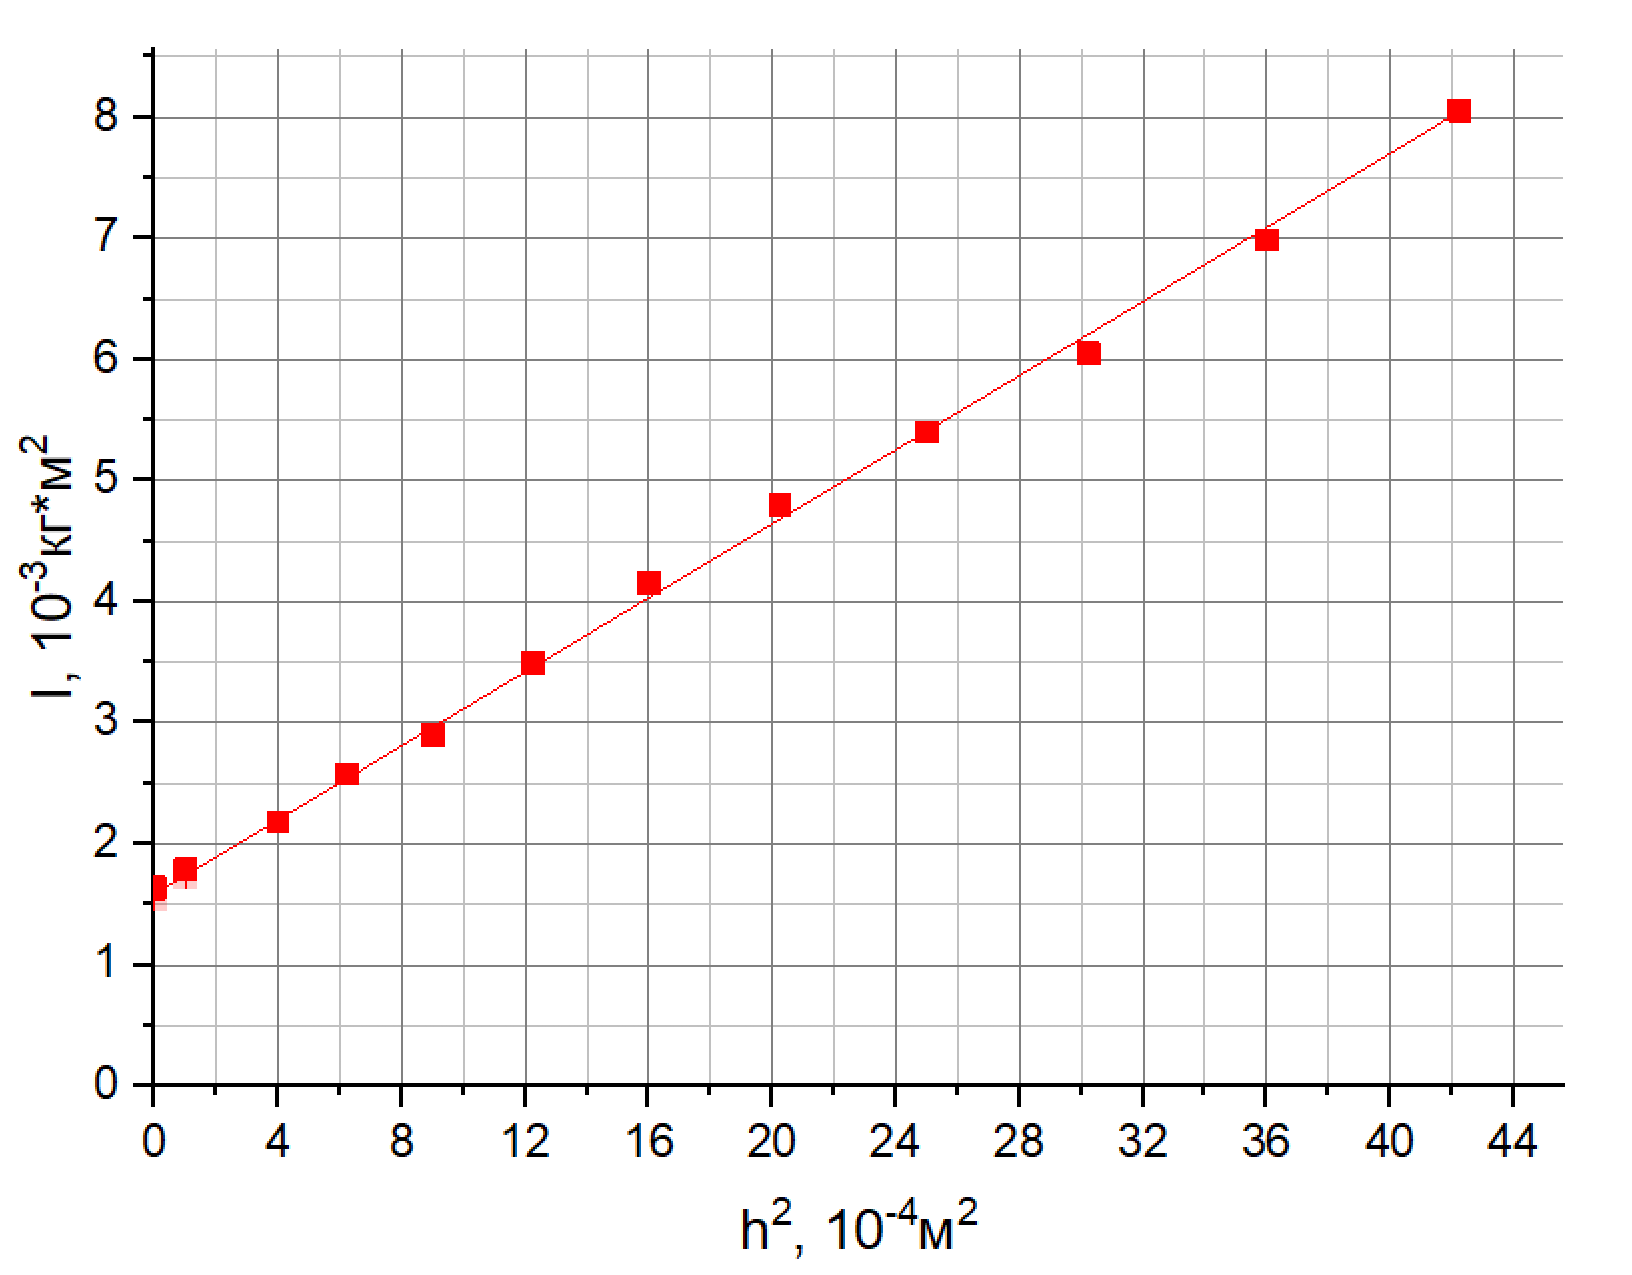
\includegraphics[scale=0.36]{4}
\caption{График зависимости момента инерции двух полуцилиндров $I$ от расстояния в квадрате $h^2$}
\end{figure}
\section{Обсуждение результатов и выводы}
В работе экспериментально были получены моменты инерции полого цилиндра, диска и системы: диск+цилиндр соответственно:
\[I_\text{ц} = (6,58\pm 0,26)\text{г}\cdot \text{м}^2\]
\[I_\text{д} = (2,02\pm 0,22)\text{г}\cdot \text{м}^2\]
\[I_\text{д+ц} = (8,8\pm 0,3)\text{г}\cdot \text{м}^2\]
Также были посчитаны моменты инерции полого цилиндра и диска по теоретическим формулам (погрешность пренебрежимо мала):
\[I_\text{ц}^\text{т} = 6,8\text{г}\cdot \text{м}^2\]
\[I_\text{д}^\text{т} = 2,1\text{г}\cdot \text{м}^2\]
По результатам, можно сделать вывод, что теоретические значения сошлись с экспериментальными.

Также выполняется соотношение:
\[I_\text{ц}+I_\text{д} = (8,6\pm 0,5)\text{г}\cdot \text{м}^2\approx (8,8\pm 0,3)\text{г}\cdot \text{м}^2 =  I_\text{д+ц} \]
Что подтверждает аддитивность момента инерции. 

Во второй части работы была проведена проверка теоремы Гюйгенса-Штейнера:
\[I = I_c + mR^2\]
$I$ -- момент инерции тела относительно оси, параллельной оси, проходящей через центр масс и удаленной от нее на расстояние $R$\\
$I_c$ -- момент инерции тела относительно оси, проходящей через центр масс\\
$m$ -- масса тела

График зависимостм момента инерции двух полуцилиндров $I$ от расстояния в квадрате $h^2$ (Рис. 3) отражает линейную зависимость между этими величинами, что соответствует теореме Гюйгенса-Штейнера.
\end{document}